\documentclass{scrreprt}

% packages
\usepackage{amsmath}
\usepackage[margin=0.8in]{geometry}
\usepackage{graphics}
\usepackage{graphicx}
\usepackage[round]{natbib}
\usepackage{pst-node}
\usepackage[hyphens,obeyspaces]{url}

% settings
\bibliographystyle{plainnat}
\setkomafont{sectioning}{\normalfont\bfseries}
\newenvironment{denseitem}{
  \begin{itemize}
    \setlength{\itemsep}{0pt}
    \setlength{\parskip}{0pt}
    \setlength{\parsep}{0pt}
}{
  \end{itemize}
}

\title{Evapotranspiration Modeling in ECHSE: Documentation}
\author{Julius Eberhard}

%::::::::::::::::::::::::::::::::::::::::::::::::::::::::::::::::::::::::::::::::

\begin{document}

\maketitle
\tableofcontents

%................................................................................

\chapter{Introduction} \label{ch:introduction}

This is a documentation of my work done in exploring some aspects of the way how evapotranspiration is simulated in the \emph{Eco-Hydrological Simulation Environment} (ECHSE, \citealt{kneis15}) with methods, classes, and engines written by Tobias Pilz.
ECHSE is a model framework, i.e. a software providing calculation methods that can be composed modularly to form model engines. These engines can be compiled and be run as independent models with input data.
ECHSE is used in the field of (eco-) hydrology and therefore comes with a collection of methods especially relevant for issues in this field.
The goal of the bigger project is to apply with ECHSE different models for determining the potential ($et_{pot}$) and the actual evapotranspiration ($et_{act}$).
These are, as of the date of this documentation:
\begin{denseitem}
  \item[--] the model of \citet{makkink57},
  \item[--] the model of Penman and Monteith \citep{monteith65},
  \item[--] the model of Penman and Monteith as simplified by the FAO \citep{fao98},
  \item[--] the model of \citet{shuttleworth85}.
\end{denseitem}

The engine-specific names (identifiers) of variables and parameters are written in \verb!fixed-width! whereas the physical symbols of variables, constants, and parameters are written in \textit{italics}.
E.g., extraterrestrial radiation = $R_{ex}$ = \verb!radex!.
Terms that describe parts of the ECHSE architecture are written in \textsf{sans-serif}.

\section{Overview of models, engines, parameters} \label{sec:intro_overview}

\textbf{Models.}
The physical $et$ models implemented in ECHSE originated from two approaches:
First, the empirical approach of \citet{makkink57} as simplified by \citet{debruin87} (for applications during the growing season) uses global radiation (explicitly), air pressure (implicitly through the use of the psychrometric `constant'), and temperature (implicitly through the use of the slope of the saturated vapor pressure curve and the psychrometric `constant') as predictors for the potential evapotranspiration.
Secondly, the consideration of the net energy available for evaporating water from an open water surface was incorporated into earlier empirical findings by Penman and supplemented with the concept of surface and aerodynamical resistances for uniformly vegetated and completely covered ground by \citet{monteith65} to form the Penman-Monteith model.
For a nice overview of the Makkink (Makk) and the Penman-Monteith (PM) model and how they are theoretically related, see \citet{debruin87}.

The widely used PM formula was later simplified for rough estimates of single crops by the Food and Agriculture Organization of the United Nations FAO \citep{fao98} (FAO model) and improved for sparse crops by \citet{shuttleworth85} (SW model).

Tab.~\ref{tab:models} gives a very brief overview of the four models.
It contains keywords describing the way how a type of $et$ is simulated in the respective ECHSE engine.
\emph{Reference} $et$ quantifies the evapotranspiration from reference surfaces which usually are made of densely growing, clipped grass which always has a sufficient water supply for transpirating at a maximum rate.
\emph{Potential} $et$ is the maximum possible evapotranspiration from a certain (not necessarily reference) surface which also has no limited water supply.
\emph{Actual} $et$ takes into account factors that limit the water supply.
E.g., potential $et$ in the Makk model is calculated by multiplying the reference $et$ with a crop factor while the potential $et$ is multiplied with a soil moisture factor for determining the actual $et$.

%Makkink:
%\begin{align}
%  et_{ref} = 0.26 \frac{s}{s + \gamma} \frac{R_{inS}}{1000 \times E_{wat} \rho_w}
%\end{align}
%
%Penman-Monteith:
%\begin{align}
%  et_{pot} = \frac{1}{E_{wat}} \frac{s(R_{net}-G_{soil})+\rho_{air} C_{air}(E - e)/r_{aa}}{s+\gamma(1+r_{cs}/r_{aa})}
%\end{align}
%
%FAO:
%\begin{align}
%  
%\end{align}
%
\begin{table}[ht]
  \caption{Overview of $et$ models.}
  \centering
  \begin{tabular*}{1.0\hsize}{llll}
    Model & Reference $et$  & Potential $et$                             & Actual $et$ \\
    \hline
    Makk  & Makkink formula & $\times$ crop factor                       & $\times$ soil moisture factor \\
    PM    & ---             & PM formula, resistances w/o stress factors & PM, res. w/ stress \\
    FAO   & FAO formula     & $\times$ crop factor                       & $\times$ soil moisture factor \\
    SW    & ---             & SW formula, resistances w/o stress factors & SW, res. w/ stress \\
  \end{tabular*}
  \label{tab:models}
\end{table}

\textbf{Engines.}
All possibilities regarding the type of evapotranspiration (potential or actual), the model (Makk, PM, FAO, or SW), and other calculation methods are generally included in one engine.
The engine requires the user to choose between the possible combinations of methods and follows them through the calculation process.
Thus it is possible to directly compare the outputs of different methods with the same set of parameters which is supplied by the user.

\textbf{Parameters.}
The engine parameters can be grouped into
\begin{denseitem}
  \item[--] aerodynamic parameters,
  \item[--] geographical parameters,
  \item[--] radiation parameters,
  \item[--] soil hydraulic parameters,
  \item[--] vegetation parameters,
\end{denseitem}
%
according to their physical role, and will be discussed in this order in Ch.~\ref{ch:parest}.
Within the ECHSE engines, parameters are grouped into the types
\begin{denseitem}
  \item[--] \textsf{paramNum} (object-specific scalar parameters),
  \item[--] \textsf{sharedParamNum} (group-specific scalar parameters),
  \item[--] \textsf{inputExt} (group-specific time-dependent scalar parameters treated as external input variables),
\end{denseitem}
%
according to their role in the computation process.
Tab.~\ref{tab:varpar} contains an overview of the variables and parameters and whether they are used in the different $et$ models.
The parameters in this overview are grouped into the types \textsf{paramNum}, \textsf{sharedParamNum}.
Parameters of the \textsf{inputExt} type can be found together with the actual external input variables.

\begin{table}[ht]
  \caption{External input variables, parameters and their usage in the $et$ models.
           For abbreviations, see text.
           \textbullet: required by engine primarily, $\circ$: required only in cases when some primary input is missing.}
  \scalebox{0.7}{%
    \begin{tabular*}{0.70\hsize}{|cccc|ccc|r|}
      \hline
      \multicolumn{4}{c}{$et_{pot}$}                                & \multicolumn{3}{c}{$et_{act}$}  & \\
      Makk          & PM            & FAO           & SW            & PM          & FAO & SW          & ECHSE identifier \\
      \hline
                    &               &               &               &             &     &             & \textbf{\textsf{inputExt}} \\
                    & $\circ$       & $\circ$       & $\circ$       &             &     &             & \texttt{alb} \\
      \textbullet   & \textbullet   & \textbullet   & \textbullet   &             &     &             & \texttt{apress} \\
                    & \textbullet   &               & \textbullet   &             &     &             & \texttt{cano\_height} \\
      $\circ$       & $\circ$       & $\circ$       & $\circ$       &             &     &             & \texttt{cloud}* \\
      $\circ$       & $\circ$       & $\circ$       & $\circ$       &             &     &             & \texttt{doy} \\
      \textbullet   & \textbullet   & $\circ$       & \textbullet   &             &     &             & \texttt{glorad} \\
                    & $\circ$       & $\circ$       & $\circ$       &             &     &             & \texttt{glorad\_max} \\
      $\circ$       & $\circ$       & $\circ$       & $\circ$       &             &     &             & \texttt{hour} \\
                    & \textbullet   &               & \textbullet   &             &     &             & \texttt{lai} \\
                    & $\circ$       & $\circ$       & $\circ$       &             &     &             & \texttt{rad\_long} \\
                    & \textbullet   & \textbullet   & \textbullet   &             &     &             & \texttt{rad\_net} \\
                    & $\circ$       & $\circ$       & \textbullet   &             &     &             & \texttt{rad\_net\_soil} \\
                    & \textbullet   & \textbullet   & \textbullet   &             &     &             & \texttt{rhum} \\
                    & \textbullet   &               & \textbullet   &             &     &             & \texttt{soilheat} \\
      $\circ$       & $\circ$       & $\circ$       & $\circ$       &             &     &             & \texttt{sundur} \\
      $\circ$       & $\circ$       & $\circ$       & $\circ$       &             &     &             & \texttt{temp\_max} \\
      $\circ$       & $\circ$       & $\circ$       & $\circ$       &             &     &             & \texttt{temp\_min} \\
      \textbullet   & \textbullet   & \textbullet   & \textbullet   &             &     &             & \texttt{temper} \\
                    &               &               & \textbullet   &             &     &             & \texttt{totalheat} \\
      $\circ$       & $\circ$       & $\circ$       & $\circ$       &             &     &             & \texttt{utc\_add} \\
                    &               &               &               &             &     &             & \texttt{wc\_vol\_root} \\
                    &               &               &               &             &     &             & \texttt{wc\_vol\_top} \\
                    & \textbullet   & \textbullet   & \textbullet   &             &     &             & \texttt{wind} \\
      \hline
                    &               &               &               &             &     &             & \textbf{\textsf{paramNum}} \\
                    & \textbullet   &               & \textbullet   &             &     &             & \texttt{bubble} \\
                    &               & \textbullet   &               &             &     &             & \texttt{crop\_faoref} \\
      \textbullet   &               &               &               &             &     &             & \texttt{crop\_makk} \\
      $\circ$       & $\circ$       & $\circ$       & $\circ$       &             &     &             & \texttt{elev} \\
                    & \textbullet   &               & \textbullet   &             &     &             & \texttt{glo\_half} \\
      $\circ$       & $\circ$       & $\circ$       & $\circ$       &             &     &             & \texttt{lat} \\
                    & $\circ$       & $\circ$       & $\circ$       &             &     &             & \texttt{lon} \\
                    &               &               &               & \textbullet &     & \textbullet & \texttt{par\_stressHum} \\
                    &               &               &               & \textbullet &     & \textbullet & \texttt{pores\_ind} \\
                    & \textbullet   &               & \textbullet   &             &     &             & \texttt{res\_leaf\_min} \\
                    &               &               & \textbullet   &             &     &             & \texttt{soil\_dens} \\
                    &               &               &               &             &     &             & \texttt{wc\_etmax} \\
                    &               &               &               &             &     &             & \texttt{wc\_pwp} \\
                    &               &               &               &             &     &             & \texttt{wc\_res} \\
                    &               &               &               &             &     &             & \texttt{wc\_sat} \\
                    &               &               &               &             &     &             & \texttt{wstressmax} \\
                    &               &               &               &             &     &             & \texttt{wstressmin} \\
      \hline
                    &               &               &               &             &     &             & \textbf{\textsf{sharedParamNum}} \\
      \textbullet   & \textbullet   & \textbullet   & \textbullet   &             &     &             & \texttt{choice\_et} \\
                    & $\circ$       & $\circ$       & $\circ$       &             &     &             & \texttt{choice\_gloradmax} \\
                    & \textbullet   &               & \textbullet   &             &     &             & \texttt{choice\_plantDispl} \\
                    & \textbullet   &               & \textbullet   &             &     &             & \texttt{choice\_rcs} \\
                    & \textbullet   &               & \textbullet   &             &     &             & \texttt{choice\_roughLen} \\
                    & \textbullet   &               & \textbullet   &             &     &             & \texttt{drag\_coef} \\
                    &               &               & \textbullet   &             &     &             & \texttt{eddy\_decay} \\
                    & $\circ$       & $\circ$       & $\circ$       &             &     &             & \texttt{emis\_a} \\
                    & $\circ$       & $\circ$       & $\circ$       &             &     &             & \texttt{emis\_b} \\
                    & \textbullet   &               & \textbullet   &             &     &             & \texttt{ext} \\
                    & $\circ$       & $\circ$       & \textbullet   &             &     &             & \texttt{f\_day} \\
                    & $\circ$       & $\circ$       & \textbullet   &             &     &             & \texttt{f\_night} \\
                    & $\circ$       & $\circ$       & $\circ$       &             &     &             & \texttt{fcorr\_a} \\
                    & $\circ$       & $\circ$       & $\circ$       &             &     &             & \texttt{fcorr\_b} \\
                    & \textbullet   &               &               &             &     &             & \texttt{h\_humMeas} \\
                    & \textbullet   &               &               &             &     &             & \texttt{h\_tempMeas} \\
                    & \textbullet   & \textbullet   & \textbullet   &             &     &             & \texttt{h\_windMeas} \\
      $\circ$       & $\circ$       & $\circ$       & $\circ$       &             &     &             & \texttt{radex\_a} \\
      $\circ$       & $\circ$       & $\circ$       & $\circ$       &             &     &             & \texttt{radex\_b} \\
                    &               &               & \textbullet   &             &     &             & \texttt{res\_b} \\
                    & \textbullet   &               & \textbullet   &             &     &             & \texttt{rough\_bare} \\
                    &               &               & \textbullet   &             &     &             & \texttt{rss\_a} \\
                    &               &               & \textbullet   &             &     &             & \texttt{rss\_b} \\
      \hline
                    &               &               &               &             &     &             & *\emph{currently not used} \\
      \hline
    \end{tabular*}%
  }
  \label{tab:varpar}
\end{table}

In Ch.~\ref{ch:results}, an overview of the estimated parameter values is given, grouped into the \textsf{paramNum}, \textsf{sharedParamNum}, and \textsf{inputExt} parameter types.

\section{Study areas -- available data} \label{sec:intro_areas}

\subsection{Portugal} \label{ssec:intro_areas_portugal}

The \emph{Herdade da Machuqueira do Grou} area is a 2,500~ha sized woodland in the Santar\'em district, between the towns of Coruche and Foros do Arr$\tilde{\text{a}}$o, Portugal.
The vegetation is dominated by cork oak trees and shrubs.
A part of the meteorological data comes from two measurement stations within the woodland.
One station is located between trees under the open sky (\emph{Hauptstation}, HS), the other was set up under a cork oak (\emph{Nebenstation A}, NSA).
The data for both stations include
\begin{denseitem}
  \item[--] incoming short-wave radiation,
  \item[--] outgoing (reflected) short-wave radiation,
  \item[--] incoming long-wave radiation,
  \item[--] outgoing long-wave radiation,
  \item[--] air temperature,
  \item[--] soil heat flux,
  \item[--] soil moisture content,
  \item[--] sensible heat flux,
  \item[--] latent heat flux,
  \item[--] vapor pressure deficit,
  \item[--] vapor pressure,
  \item[--] wind speed;
\end{denseitem}
%
they were recorded hourly.
An evaporation flux was determined through the use of the Bowen ratio, i. e. the ratio of sensible to latent heat flux.

Additional meteorological data come from an eddy-covariance tower in the area (set up at UTM coordinates 557,689.5 easting, 4,332,375.0 northing; NSB\_TOWER in Fig.~\ref{fig:map_coruche}).
They include
\begin{denseitem}
  \item[--] net short-wave radiation,
  \item[--] net long-wave radiation,
  \item[--] air temperature,
  \item[--] relative humidity,
  \item[--] rainfall,
  \item[--] atmospheric pressure;
\end{denseitem}
%
they were recorded half-hourly.

\begin{figure}[ht]
  \centering
  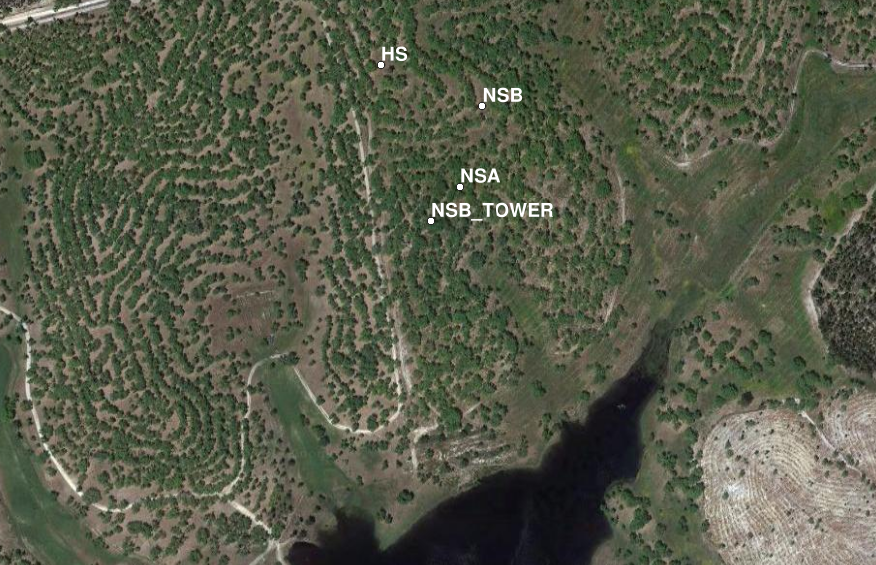
\includegraphics[width=0.7\hsize]{./map_coruche}
  \caption{Satellite image (\emph{Google Maps}) of the study area in Portugal with locations of the field stations (HS, NSA) and the eddy-covariance tower (NSB\_TOWER).}
  \label{fig:map_coruche}
\end{figure}


\subsection{Morocco} \label{ssec:intro_areas_morocco}

The study area is a citrus orchard near the village Ait Cheikh, southwest of Marrakesh, lying in the Haouz plain north of the Atlas mountains \citep{mroos14}.
The available data contain
\begin{denseitem}
  \item[--] relative humidity,
  \item[--] global radiation,
  \item[--] air temperature,
  \item[--] wind speed,
  \item[--] latent heat;
\end{denseitem}
%
they were recorded (latent heat: calculated?) half-hourly.
An evaporation flux was determined from energy balance considerations.

Additionally, soil data were taken from \citet{mroos14}.

%................................................................................

\chapter{Aims} \label{ch:aims}

The aims of my work are:
\begin{itemize}
  \item[--] the estimation of engine parameters through transfer functions and model calibration (Ch.~\ref{ch:parest}),
  \item[--] comparison of the different evapotranspiration models (Ch.~\ref{ch:modelcomp}),
  \item[--] sensitivity analysis of engine parameters (Ch.~\ref{ch:sensana}),
  \item[--] evaluation of single methods employed in the $et$ models (Ch.~\ref{ch:methodcomp}).
  \item[--] Which input data do we still need? (Ch.~\ref{ch:conclusion})
\end{itemize}

%................................................................................

\chapter{Parameters: methods and results} \label{ch:parest}

The estimation of \textbf{aerodynamic parameters}, which specify the aerodynamic resistances in the PM and the SW models, was mostly not possible in the study cases and therefore adopted from the original publications.
Nevertheless, the origins of the values are discussed briefly (Sec.~\ref{sec:parest_aero}).

\textbf{Geographical parameters} were given or easy to estimate from map services (Sec.~\ref{sec:parest_geo}).

\textbf{Radiation parameters} were partly estimated from observations of radiation components at the study sites and are discussed more extensively (Sec.~\ref{sec:parest_rad}).

Two pedotransfer functions (PTF) were used to estimate \textbf{soil hydraulic parameters} from the measured soil properties, namely bulk density, mass portions of silt and clay, and organic matter content (Sec.~\ref{sec:parest_soil}).

All \textbf{vegetation parameters} were adapted from other publications or estimated through model calibration (Sec. \ref{sec:parest_veg}).
They are discussed in separate sections to specify the problems and possibilities relevant for their determination.

Where parameters appear in their own sections, the discussion follows the outline \emph{Basics -- Methods -- Notes -- Portugal -- Morocco}.

\section{Aerodynamic parameters} \label{sec:parest_aero}

All estimated or adopted values were employed for both Portugal and Morocco because the aerodynamic conditions are similar.

Below the canopy toward the ground, wind speed is assumed to decrease exponentially with a scaling coefficient $n$, called the \textbf{eddy diffusivity decay constant} (\verb!eddy_decay!); more precisely:
The shearing stress of wind on a horizontal plane is proportional to $\rho \partial u / \partial z$ (where $u$ is the horizontal wind component, $z$ the vertical coordinate, and $\rho$ the density of air) with the proportionality factor $K$.
$n$ relates the magnitude of $K$ at the canopy height to that at the ground.
\citet{shuttleworth85} use a value of $n = 2.5$, arguing that it results from the crop specification made by \citet{monteith73} in deriving the above relation.
Although I couldn't reconstruct this value from the second edition of Monteith's book \citep{monteith90}, \citet{shuttleworth85} concluded from an sensitivity analysis that the resulting evapotranspiration was hardly influenced by changing $n$.
Therefore, $n$ has been set to 2.5.

The \textbf{measurement heights of relative humidity} (\verb!h_humMeas!), \textbf{temperature} (\verb!h_tempMeas!), and \textbf{wind speed} (\verb!h_windMeas!) are known from the measurement setups and each equal to 2~m in Portugal as well as in Morocco.

The aerodynamic \textbf{mean boundary layer resistance} $r_b$ (\verb!res_b!) was taken as 25~s~m$^{-1}$ by \citet{shuttleworth85} based on field measurements by \citet{denmead76} and \citet{uchijima76}.
Like for $n$, the models seem to be quite insensitive for variations of $r_b$ \citep{shuttleworth85}, and $r_b$ has been set to 25~s~m$^{-1}$.

In the calculation of the aerodynamic resistance between canopy and reference level, the displacement height of the vegetation and the roughness lengths for latent and sensible heat fluxes of the vegetation are used (see Sec. \ref{sec:parest_veg} for these parameters).
Following \citet{shuttleworth90}, both of these are dependent on the \textbf{roughness length of the bare substrate} $z_0$ (\verb!rough_bare!) and the effective mean \textbf{drag coefficient of the vegetation} $c_d$ (\verb!drag_coef!) as well as on the leaf area index and the canopy height (Sec. \ref{sec:parest_veg}).
The values of $z_0$ and $c_d$ were numerically estimated by the authors and are adopted here as 0.01~m and 0.07, respectively.

\section{Geographical parameters} \label{sec:parest_geo}

Each model employs 3 or less geographical parameters for calculating the radiation balance: \textbf{latitude} $\varphi$ (\verb!lat!), \textbf{longitude} $L_m$ (\verb!lon!), \textbf{elevation} $h$ (\verb!elev!).
For the sites in Portugal, the locations were given as UTM coordinates (HS: 557,640.5~m easting, 4,332,523.5~m northing; NSA: 557,717.0~m easting, 4,332,408.0~m northing; both in UTM zone~29S) from which I could derive $\varphi = 39.14^\circ$~N and $L_m= 8.33^\circ$~W for both field stations.
The actual distance of 139~m between the stations corresponds to less than $0.01^\circ$ and was therefore taken as 0.
A common value for $h$ of the Portugal sites was estimated from local elevation maps (\emph{floodmap.net}) as 160~m above sea level.

For Morocco, $\varphi = 31.50^\circ$~N, $L_m = 8.14^\circ$~W, and $h = 464$~m~a.s.l. were taken from \citet{mroos14}.

\section{Radiation parameters} \label{sec:parest_rad}

\subsection{Albedo (\texttt{alb})} \label{ssec:parest_rad_alb}

\textbf{Basics.}
The albedo $\mu$ (\verb!alb!) is defined as
\begin{align*}
  \mu = \frac{R_{outS}}{R_{inS}}
\end{align*}
%
with
\begin{denseitem}
  \item[] $R_{outS}$: outgoing short-wave radiation, in W~m$^{-2}$,
  \item[] $R_{inS}$: incoming short-wave radiation (\verb!glorad!), in W~m$^{-2}$.
\end{denseitem}

\textbf{Method.}
It can be estimated from observations of $R_{inS}$ and $R_{outS}$ or from literature values for various land surfaces.
The albedo of a surface can change over time and is supplied as a time series in ECHSE.

\textbf{Portugal.}
The measurements of the short-wave radiation components at the stations HS and NSA comprised hourly time series between April 7 and August 4, 2014.
The albedo was derived as a total mean of the hourly $R_{outS}/R_{inS}$ ratio.
Only records of times between 8:00 and 16:00 were used for the estimation.
Although the observations showed a distinct development over time (Fig.~\ref{fig:portugal_alb}), I could not conclude the amplitude of yearly fluctuations from the observations and therefore used the calculated mean as a constant value over the whole year, $\mu = 0.066$.

\begin{figure}[ht]
  \centering
  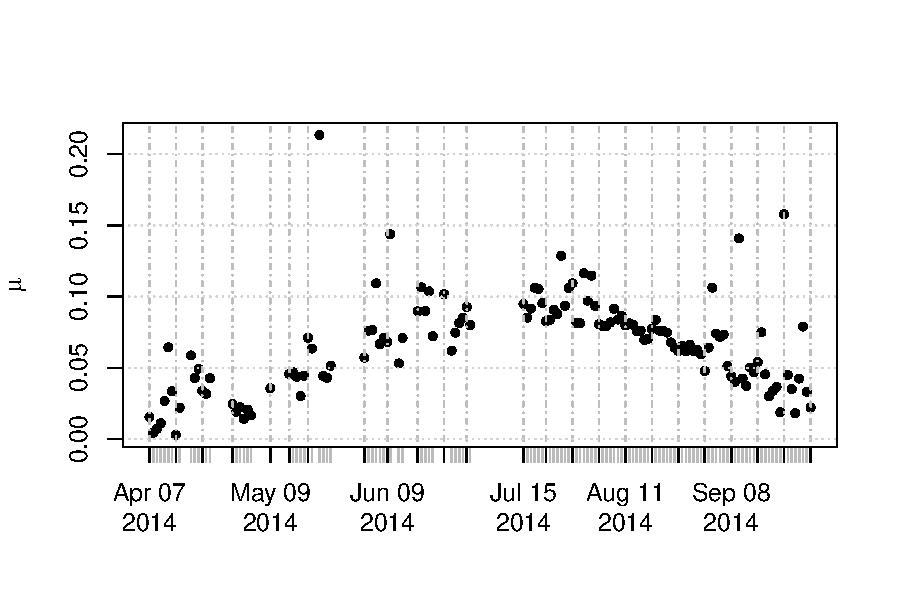
\includegraphics[width=0.6\hsize]{./plot_alb.pdf}
  \caption{$R_{outS}/R_{inS}$ ratio, daily mean. Total mean: $\mu = 0.0816$.}
  \label{fig:portugal_alb}
\end{figure}

\textbf{Morocco.}
None of the measurements did include $R_{outS}$ data, so the albedo has been estimated as constantly 0.3, judging by the descriptions of the surfaces.
These are likely to have $0.25 < \mu < 0.4$, where 0.25 is the albedo of green grass \citep{markvart03} and 0.4 that of dry sand \citep{tetzlaff83}.

\subsection{Emissivity parameters (\texttt{emis\_a}, \texttt{emis\_b})} \label{ssec:parest_rad_emis}

\textbf{Basics.}
Emissivity is a property of a macroscopic body (fluid or solid) and gives the portion of radiation that the body emits compared with a black body at the same temperature.
There are two methods for calculating the net emissivity $\varepsilon$ between Earth's surface and atmosphere in ECHSE, either from water vapor pressure (Eq.~\ref{eq:emis1}) or from air temperature (Eq.~\ref{eq:emis3}).
The first method includes the emissivity parameters $\varepsilon_a$, $\varepsilon_b$ (\verb!emis_a!, \verb!emis_b!), which represent the average environmental effects (such as surface and climate) on $\varepsilon$ at a certain location \citep{brunt32}:
\begin{align} \label{eq:emis1}
  \varepsilon = \varepsilon_a + \varepsilon_b \sqrt{e}
\end{align}
%
with
\begin{denseitem}
  \item[] $\varepsilon$: net emissivity, no unit,
  \item[] $\varepsilon_a$: emissivity parameter a, no unit,
  \item[] $\varepsilon_b$: emissivity parameter b, in hPa$^{-1/2}$,
  \item[] $e$: water vapor pressure in air, in hPa.
\end{denseitem}
%
$e$ is derived from measurements of the air temperature and the relative humidity.
$\varepsilon$ itself is used in ECHSE for the calculation of the net incoming long-wave radiation (adapted Stefan-Boltzmann law):
\begin{align} \label{eq:emis2}
  L_n = -f \varepsilon \sigma (TA + 273.15~\text{K})^4
\end{align}
%
with
\begin{denseitem}
  \item[] $L_n$: net incoming long-wave radiation, in W~m$^{-2}$~K$^{-4}$,
  \item[] $f$: cloudiness correction factor (Sec.~\ref{ssec:parest_rad_fcorr}), no unit,
  \item[] $\varepsilon$: net emissivity between ground and atmosphere, no unit,
  \item[] $\sigma$: Stefan-Boltzmann constant, $5.670373 \times 10^{-8}$~W~m$^{-2}$~K$^{-4}$,
  \item[] ${TA}$: mean air temperature, in $^\circ$C.
\end{denseitem}

\textbf{Method.}
The parameters $\varepsilon_a$, $\varepsilon_b$ can be estimated through Eqs.~\eqref{eq:emis2} and \eqref{eq:emis1} if sufficient data of $L_n$, $TA$, $e$, and $f$ are available.
If not, one can look up suggested values by \citet{maidment93} (p.~4.7), i. e. $\varepsilon_a = 0.34$ and $\varepsilon_b = -0.14$ for ``average conditions'' and general ranges of 0.34 to 0.44 for $\varepsilon_a$ and $-0.14$ to $-0.25$ for $\varepsilon_b$, derived from data in \citet{fao77}.

\textbf{Note.}
The second method for calculating $\varepsilon$ uses air temperature as the only predictor for $\varepsilon$ without the need of $\varepsilon_a$, $\varepsilon_b$, $e$ and was published in \citet{maidment93} based on \citet{idso69}:
\begin{align} \label{eq:emis3}
  \varepsilon = -0.02 + 0.261 \exp(-7.77 \times 10^{-4} TA^2)
\end{align}
%
with
\begin{denseitem}
  \item[] $TA$: mean air temperature, in $^\circ$C.
\end{denseitem}
%
It seems that Eq.~\eqref{eq:emis1} is the more suitable choice if $e$ is known since it lets the user implement more of the specific environmental conditions at a study site through the emissivity parameters.
However, if $\varepsilon_a$ and $\varepsilon_b$ can't be determined as explained and both $e$ and $TA$ data are available, the question is whether it is better to use Eq.~\eqref{eq:emis1} with average-condition values from \citet{maidment93} or Eq.~\eqref{eq:emis3}.
ECHSE prefers Eq.~\eqref{eq:emis1} as soon as any $e$ data are given as an input and thereby follows the recommendation of \citet{maidment93}.
As can be seen in Sec.~\ref{ssec:parest_rad_fcorr}, the cloudiness correction factor $f$ is determined by two parameters ($f_a$, $f_b$), which need to be supplied by the user.
Their estimation is possible only through the use of Eq.~\eqref{eq:emis2}, thus dependent on $\varepsilon$ data.
This means that a well-founded calculation of the emissivity is the requirement for a good estimation of $f_a$ and $f_b$.
Since it was not clear which method would provide a better value of $\varepsilon$, I decided to use both methods and compare the outputs of the models.
A simple sensitivity analysis indicated that the $et$ models of PM and SW could only show a small, if any, reaction to changing the emissivity model.

\textbf{Portugal.}
I chose default values of $\varepsilon_a = 0.34$ and $\varepsilon_b = -0.14$, as suggested for average conditions by \citet{maidment93}.
The values could not be estimated specifically because the cloudiness correction $f$ was not known for the study site.
Instead, $f$ was estimated with the adopted emissivity parameters through Eq.~\eqref{eq:emis2} for the determination of the cloudiness correction parameters $f_a$, $f_b$.
For a qualitative validation of the chosen values, I estimated the net emissivity from Eq.~\eqref{eq:emis2} using observations at times when global radiation was at maximum, i. e. $f \approx 1$, and compared it to the predicted values of $\varepsilon$ by both emissivity models.
Fig.~\ref{fig:portugal_emis_both} shows ``observed'' and predicted $\varepsilon$ values, distinguishing between ``noon'' hours (between 10 am and 2 pm), when $L_n$ has a maximal magnitude, and other hours of the day.
$f$ was chosen to be $0.9 < f \leq 1$.
Although some observation-derived values come near the predicted values at noon hours, both models generally overpredict the ``observed'' emissivity.

\begin{figure}[ht]
  \centering
  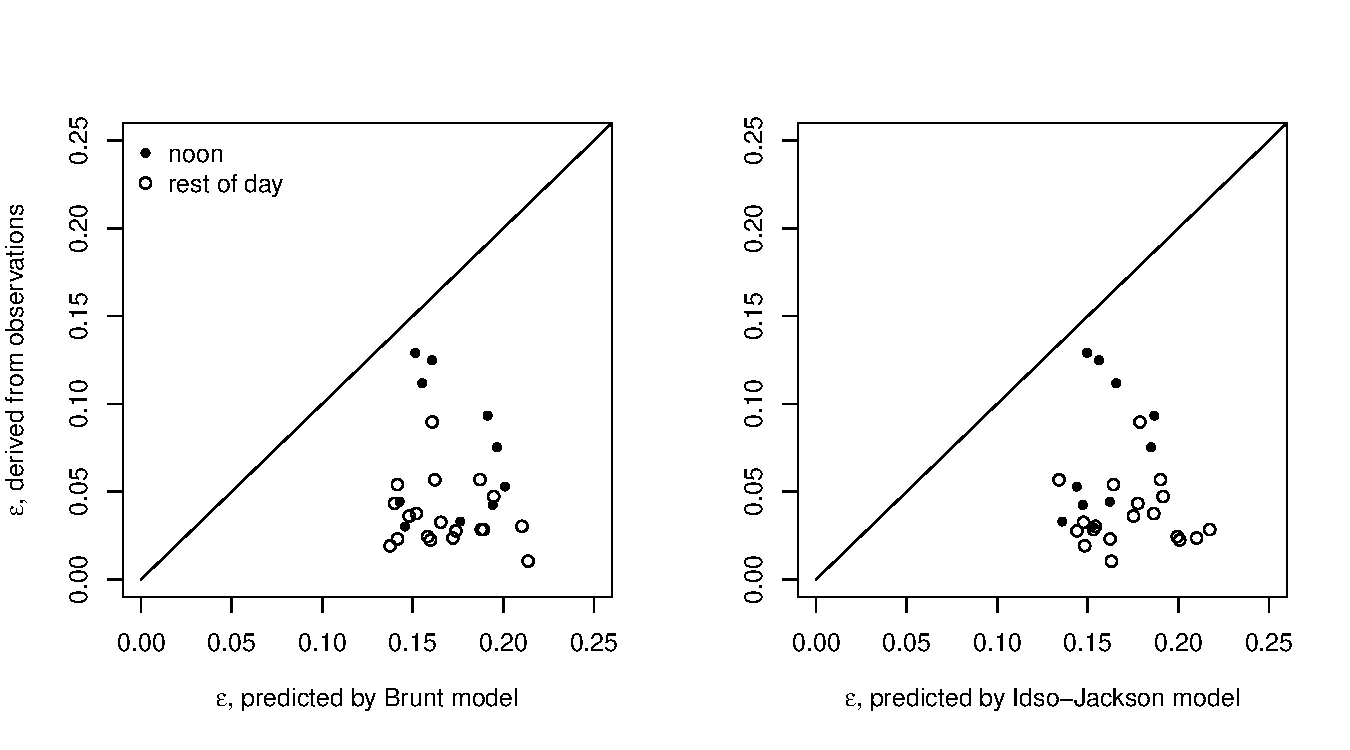
\includegraphics[width=0.8\hsize]{./plot_emis_both_HS.pdf}
  \caption{Observation-derived vs. model-predicted net emissivity at HS station.
           As $f \approx 1$ was assumed by choosing $0.9 < f \leq 1$, Eq.~\eqref{eq:emis2} is equivalent to $\varepsilon \approx - L_n / (\sigma (TA + 273.15~\text{K})^4)$ with observed $L_n$ and $TA$.}
  \label{fig:portugal_emis_both}
\end{figure}

\textbf{Morocco.}
As for Portugal, I chose $\varepsilon_a = 0.34$ and $\varepsilon_b = -0.14$.
The values could not be estimated specifically because data of the net long-wave radiation and the cloudiness correction were missing.

\subsection{Soil heat factors (\texttt{f\_day}, \texttt{f\_night})} \label{ssec:parest_rad_f}

\textbf{Basics.}
Within the ECHSE engines, the sub-daily soil heat flux is currently calculated as
\begin{align}
  G_{soil} &= f_{day} R_{net} ~ \text{during daytime}, \label{eq:f1} \\
  G_{soil} &= f_{night} R_{net} ~ \text{during nighttime}. \label{eq:f2}
\end{align}
%
with
\begin{denseitem}
  \item[] $G_{soil}$: soil heat flux (\verb!soilheat!), in W~m$^{-2}$,
  \item[] $f_{day}$, $f_{night}$: soil heat factors (\verb!f_day!, \verb!f_night!), no unit,
  \item[] $R_{net}$: net incoming short-wave and long-wave radiation (\verb!rad_net!), in W~m$^{-2}$.
\end{denseitem}

\textbf{Portugal.}
Since the data didn't include measurements of $R_{net}$, I used the results of internally calculated values of $R_{net}$ and measurements of $G_{soil}$ for calculating $f_{day}$, $f_{night}$ hourly from Eqs.~\eqref{eq:f1}, \eqref{eq:f2}.
The distinction of the time series into daytime and nighttime was made using the \emph{RAtmosphere::suncalc} procedure by Gionata Biavati, which provided sunrise and sunset times for the study site.
Averaging over all hours gave the results.

\textbf{Morocco.}
---

\subsection{Cloudiness correction parameters (\texttt{fcorr\_a}, \texttt{fcorr\_b})} \label{ssec:parest_rad_fcorr}

\textbf{Basics.}
The cloudiness correction parameters $f_a$, $f_b$ (\verb!fcorr_a!, \verb!fcorr_b!) appear as the slope and the intersect parameter of the affine relationship between the cloudiness correction factor $f$ and the relative actual global radiation:
\begin{align} \label{eq:fcorr1}
  f = f_a \frac{R_{inS}}{R_{inS,cs}} + f_b
\end{align}
%
with
\begin{denseitem}
  \item[] $f_a$, $f_b$: cloudiness correction parameters, no unit,
  \item[] $R_{inS}$: actual incoming short-wave radiation (\verb!glorad!), in W~m$^{-2}$,
  \item[] $R_{inS,cs}$: maximum possible (``clear-sky'') incoming short-wave radiation, in W~m$^{-2}$.
\end{denseitem}
%
$f$ itself is used in ECHSE for the calculation of the net incoming long-wave radiation, i.e. Eq.~\eqref{eq:emis2}:
\begin{align*}
  L_n = -f \varepsilon \sigma (TA + 273.15~\text{K})^4
\end{align*}
%
with
\begin{denseitem}
  \item[] $L_n$: net incoming long-wave radiation, in W~m$^{-2}$~K$^{-4}$,
  \item[] $\varepsilon$: net emissivity between atmosphere and ground (Sec.~\ref{ssec:parest_rad_emis}), no unit,
  \item[] $\sigma$: Stefan-Boltzmann constant, $5.670373 \times 10^{-8}$~W~m$^{-2}$~K$^{-4}$,
  \item[] $TA$: mean air temperature, in $^\circ$C.
\end{denseitem}

\textbf{Method.}
The parameters can be estimated from Eq.~\eqref{eq:emis2} if sufficient data of $L_n$, $\varepsilon$, $TA$, $R_{inS}$, and $R_{inS,cs}$ are available.
Shuttleworth gives values of $f_a = 1.35$, $f_b = -0.35$ for arid conditions and $f_a = 1.0$, $f_b = 0.0$ for humid conditions in \citet{maidment93}, p. 4.8.

\textbf{Portugal.}
First, the cloudiness correction $f$ was estimated from $L_n$, $TA$, and $\varepsilon$ where the net emissivity was calculated following both methods described in Sec.~\ref{ssec:parest_rad_emis}, i. e. Eq.~\eqref{eq:emis1} \citep{brunt32} and Eq.~\eqref{eq:emis3} \citep{idso69}.
The parameters $f_a$, $f_b$ could then be estimated through an adapted regression method:
The condition $f_a + f_b = 1$ was not possible to be fulfilled by a linear regression of $f$ over $R_{inS}/R_{inS,cs}$ (the latter of which was derived by means of the previously estimated {\AA}ngstr\"om parameters).
In order to get a model close to the data, I did a linear regression of the data (although the conditional mean didn't behave linearly and therefore did not fulfill the assumptions for a valid linear regression) and used the intersect (the value of $f$ at $R_{inS} = 0$) as estimation of $f_b$.
$f_a$ was then determined from the condition above.
Fig.~\ref{fig:portugal_fcorr} shows the calculated cloudiness correction and the adapted regression models for both emissivity methods as well as the suggested model by Shuttleworth in \citet{maidment93}.

\begin{figure}[ht]
  \centering
  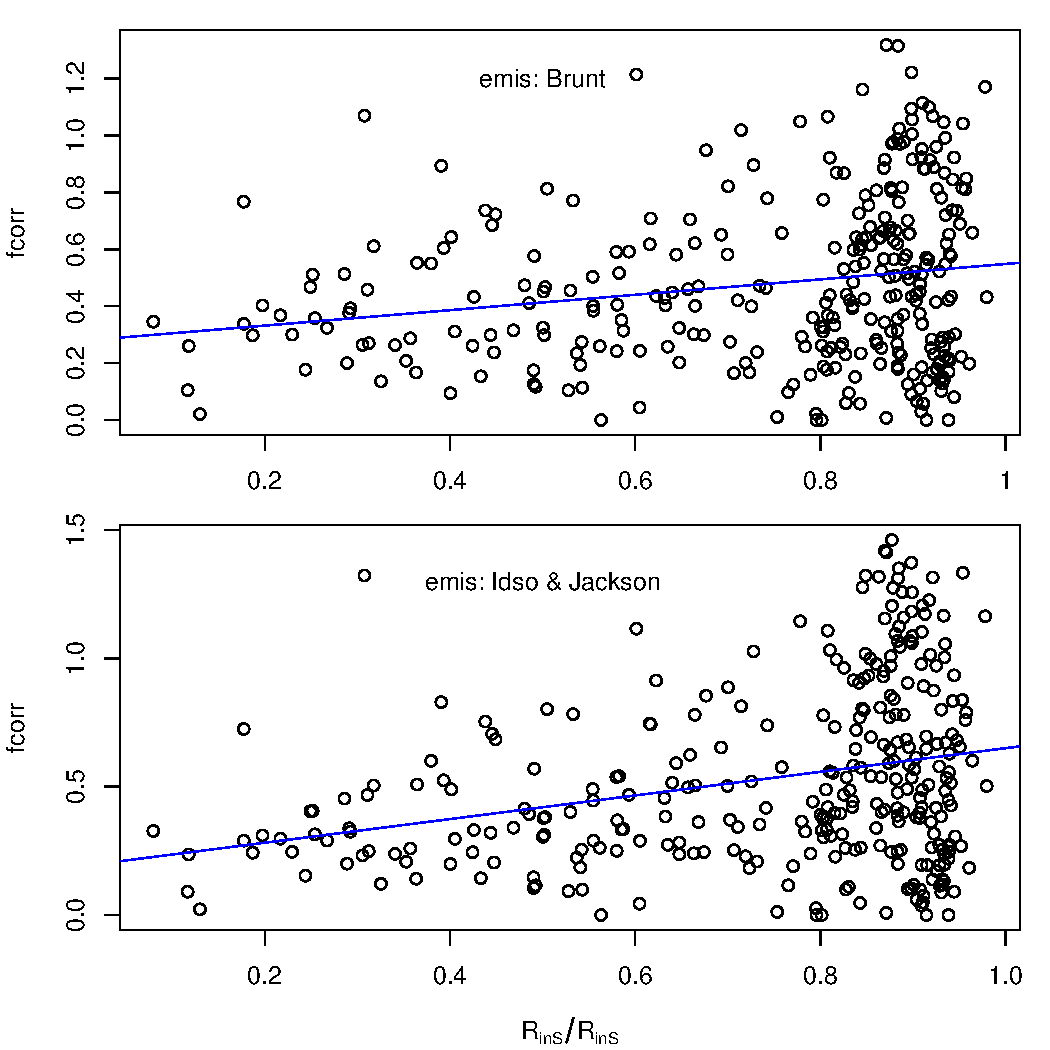
\includegraphics[width=0.6\hsize]{./plot_fcorr_both.pdf}
  \caption{Adapted regression models (lines) of hourly $f$ data (points) calculated with Eq.~\eqref{eq:emis2} for the estimation of $f_a$, $f_b$.
           See text for the regression method.
           Upper: emissivity calculated after \citet{brunt32} with $\varepsilon_a = 0.34$, $\varepsilon_b = -0.14$; lower: emissivity calculated after \citet{idso69}.}
  \label{fig:portugal_fcorr}
\end{figure}

\textbf{Morocco.}
Data of the net long-wave radiation were missing, thus I chose the suggested values for arid conditions in \citet{maidment93}.

\subsection{{\AA}ngstr\"om parameters (\texttt{radex\_a}, \texttt{radex\_b})} \label{ssec:parest_rad_radex}

\textbf{Basics.}
The estimation of the {\AA}ngstr\"om parameters is based on the equation
\begin{align} \label{eq:radex1}
  \langle R_{inS} \rangle = \left (  a_s + b_s \frac{n}{N} \right ) \langle R_{ex} \rangle,
\end{align}
%
with
\begin{denseitem}
  \item[] $\langle \cdot \rangle$: daily mean of $\cdot$,
  \item[] $R_{inS}$: incoming short-wave radiation (global radiation, \verb!glorad!), in W m$^{-2}$,
  \item[] $R_{ex}$: extraterrestrial short-wave radiation (\verb!radex!), in W m$^{-2}$,
  \item[] $a_s$, $b_s$: {\AA}ngstr\"om parameters (\verb!radex_a!, \verb!radex_b!), no unit,
  \item[] $n$: sunshine duration of current day (time for which $\langle R_{inS} \rangle \geq 120~\text{W~m}^{-2}$, \verb!sundur!), in hours,
  \item[] $N$: maximum possible sunshine duration, in hours.
\end{denseitem}

\textbf{Method 1.}
Since $R_{ex}$ and $N$ are calculated internally and astronomically based, the uncertainty of the estimation through Eq.~\eqref{eq:radex1} should only depend on the observed global radiation (by definition, $n$ follows from $R_{inS}$).
Note that the equation as written represents only daily mean values of $R_{inS}$:
The parameters are weighted depending on the daily ratio $n/N$ in order to account for cloudiness.
Two special cases are therefore
\begin{align}
  a_s + b_s &= \frac{\langle R_{inS} \rangle}{\langle R_{ex} \rangle} \text{ on days when } n=N, \label{eq:radex2} \\
  a_s &= \frac{\langle R_{inS} \rangle}{\langle R_{ex} \rangle} \text{ on days when } n=0. \label{eq:radex3}
\end{align}
%
If observations for either of these cases are available, Eqs.~\eqref{eq:radex1} \& \eqref{eq:radex2} or Eqs.~\eqref{eq:radex1} \& \eqref{eq:radex3} form a system of linear equations, i.e. the unknown parameters $a_s$, $b_s$ can be found for any given day with known values of $n$ and $R_{inS}$.
Averaging over all days would then determine the parameters.
Problem: It might be difficult to find either days when $n=N$ or days when $n=0$.

\textbf{Method 2.}
Another way of estimating $a_s$ and $b_s$ based on shorter time intervals (in our case, hourly) would be
\begin{align}
  a_s + b_s &= \max_{h = 1, ..., 24} \left \{ \frac{R_{inS} (h)}{R_{ex} (h)} \right \}, \label{eq:radex4} \\
  a_s &= \min_{h = 1, ..., 24} \left \{ \frac{R_{inS} (h)}{R_{ex} (h)} \right \} \label{eq:radex5}
\end{align}
%
with
\begin{denseitem}
  \item[] $h$: hour of day.
\end{denseitem}
%
For finding unique solutions, both Eqs.~\eqref{eq:radex4} and \eqref{eq:radex5} need to be evaluated because the equations are no longer dependent on $n$.
The biggest problem of estimating the parameters with subdaily data is that extreme values (max, min) can result from measuring errors and statistical outliers.
Taking very low quantiles of the $R_{inS}/R_{ex}$ distribution and applying an upper limit for the max ($a_s + b_s$ can't be greater than 1) would probably avoid estimating $a_s$ as too low and $b_s$ as too high.

\textbf{Portugal.}
Global radiation was measured hourly at the local weather station in Portugal.
Therefore I chose to estimate \verb!radex_a! and \verb!radex_b! with Eqs.~\eqref{eq:radex4} and \eqref{eq:radex5}.
The $R_{inS}/R_{ex}$ ratio was calculcated for daytime hours between 8:00 and 16:00 local time.
This assured that only radiation between sunrise and sunset was taken into account for all of the simulation period.
For the determination of reasonable values I chose the lower 5-percentile of the $R_{inS}/R_{ex}$ distribution as the minimum and the maximum value of $\{R_{inS}/R_{ex} < 1\}$ as the maximum over the whole period in which $R_{inS}$ observations were available.
These choices proved successful in computing clear-sky radiation that didn't exceed the observed global radiation and therefore fulfilled the physical conditions.

\begin{figure}[ht]
  \centering
  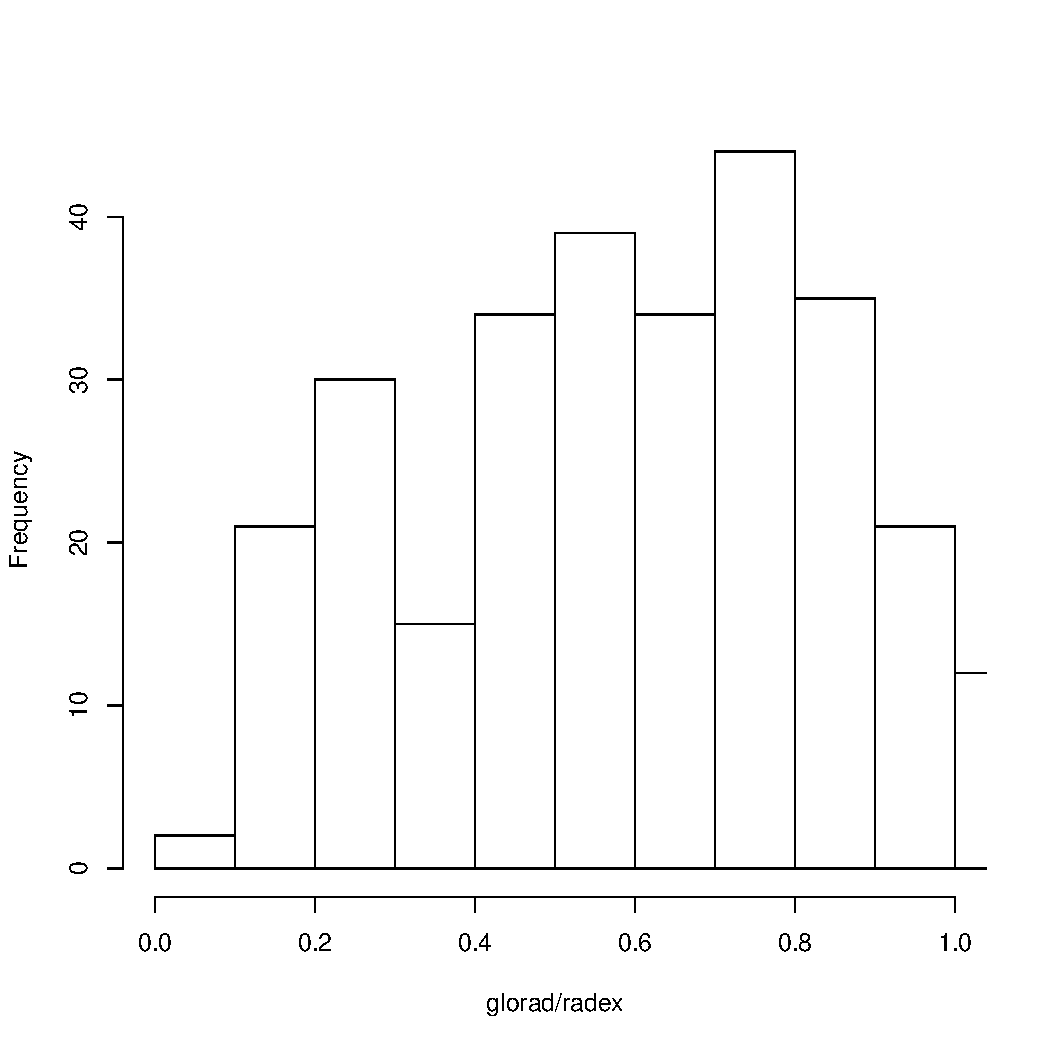
\includegraphics[width=0.5\hsize]{./plot_radex1.pdf}
  \caption{Histogram of the ratio $R_{inS}/R_{ex}$ for values less than 1 in Portugal.}
  \label{fig:portugal_radex1}
\end{figure}

\begin{figure}[ht]
  \centering
  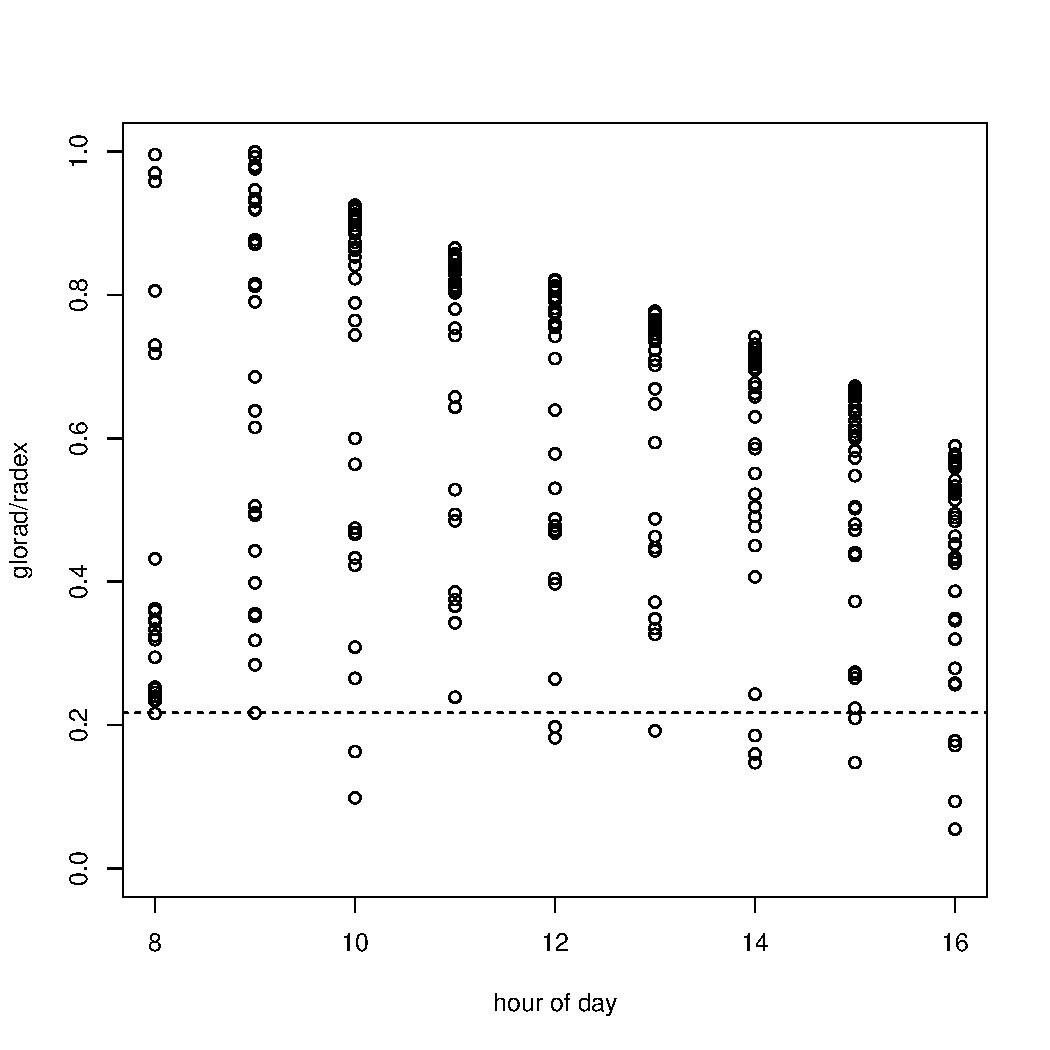
\includegraphics[width=0.6\hsize]{./plot_radex2.pdf}
  \caption{$R_{inS}/R_{ex}$ ratio dependent on hour of day.
           The shift of higher values toward early hours may indicate either a small temporal deviation between the simulated and the actual $R_{ex}$, or a local effect that weakens $R_{inS}$ during afternoon, or both.
           The dashed line marks the 5-percentile of the total distribution.}
  \label{fig:portugal_radex2}
\end{figure}

\textbf{Morocco.}
---

\section{Soil hydraulic parameters} \label{sec:parest_soil}

\verb!wc_sat!, \verb!wc_res!, \verb!wc_pwp!, \verb!wc_etmax!, \verb!bubble!, \verb!pores_ind!, \verb!wstressmin!, \verb!wstressmax!, \verb!soil_dens!, \verb!rss_a!, \verb!rss_b!.

\subsection{Capillary suction at maximum/minimum water stress (\texttt{wstressmax} / \texttt{wstressmin})}

\textbf{Basics.}
The calculation of stomatal resistance, which is required in the PM and SW models, incorporates two stress factors for vapor stress ($\Phi_{vap}$) and water stress ($\Phi_{wat}$).
The latter one relates the actual capillary suction in the soil $\psi$ (also called soil water potential) to the capillary suction at maximum ($\psi_{s,max}$) and minimum water stress ($\psi_{s,min}$) and reads
%
\begin{align*}
  \Phi_{wat} = \begin{cases}
                1, & \psi < \psi_{s,min} \\
                1 - \frac{\psi - \psi_{s,min}}{\psi_{s,max} - \psi_{s,min}}, & \psi_{s,min} \leq \psi < \psi_{s,max} \\
                0.01 & \psi \geq \psi_{s,max}
              \end{cases}
\end{align*}
%
with
\begin{denseitem}
  \item[] $\psi$: actual capillary suction, in hPa,
  \item[] $\psi_{s,max}$: capillary suction at maximum water stress (\verb!wstressmax!), in hPa,
  \item[] $\psi_{s,min}$: capillary suction at minimum water stress (\verb!wstressmin!), in hPa.
\end{denseitem}

\textbf{Method.}
Since water stress for a plant is at maximum when it is not able to detract water from the soil anymore, it's a plausible decision to set $\psi_{s,max}$ to the defined \citep{scheffer10} permanent wilting point of $10^{4.2}$~hPa.
$\psi_{s,min}$ is more difficult to determine but simple sensitivity analyses showed almost no influence of a variation of $\psi_{s,min}$ between 0 and 500~hPa (a range from full saturation to above the upper range of field capacity at $10^{2.5}$ hPa) on the simulated actual evapotranspiration.

\textbf{Portugal.}
\citet{gazdar16} measured pre-dawn capillary suctions at both study sites (HS and NSA) for different water contents.
At HS, for a minimum water content of 0.05~m$^3$~m$^{-3}$, the results were $\psi_{HS} = 1.31$~MPa for \emph{Cistus crispus} vegetation and $\psi_{HS} = 0.5$~MPa for \emph{Quercus suber}.
At NSA, for a minimum water content of 0.10~m$^3$~m$^{-3}$, $\psi_{NSA} = 1.4$~MPa for \emph{Cistus} and $\psi_{NSA} = 0.89$~MPa for \emph{Quercus}.


\textbf{Morocco.}


\section{Vegetation parameters} \label{sec:parest_veg}

\subsection{Canopy height (\texttt{cano\_height})} \label{ssec:parest_veg_canoheight}

\textbf{Basics.}
In the calculation of different aerodynamic resistances, the average canopy height of the vegetation $h_{cano}$ (\verb!cano_height!) is an important parameter.
The dependent quantities include, among others, the displacement height and the roughness length of the vegetation.

\textbf{Method.}
The canopy height can be measured in situ or estimated species- and climate-dependently from literature.

\textbf{Portugal.}
At HS, the predominant species are grasses for which I assumed a mean canopy height of 0.20~m.
At NSA, the total heights of the surrounding trees were measured.
The mean is 7.98~m for a sample size of 88 and was used as canopy height.

\subsection{FAO crop factor (\texttt{crop\_faoref})} \label{ssec:parest_veg_cropfaoref}

\textbf{Basics.}
The modified Penman-Monteith formula as published by the FAO \citep{fao98} gives a rough estimation of the potential evapotranspiration rate without the explicit use of resistances but empirically generalized factors.
The FAO crop factor (\verb!crop_faoref!), which scales the total $et$ flux, is the only parameter in the equation and specific to a site, i.e. a crop.
A value of 1 corresponds to the reference crop (well-watered grass of 0.12~m height, 70~s~m$^{-1}$ \citep{fao98} or 69~s~m$^{-1}$ \citep{shuttleworth07} surface resistance, 0.23 albedo), values for other types of vegetation can be looked up online.

\textbf{Portugal, Morocco.}
The crop factor was set to 1 for reference evapotranspiration.
Since the FAO equation is just a simplification of the Penman-Monteith equation, I preferred using the original PM model for the study cases and using the FAO reference results only for a subsumption of the different models.

\subsection{Makkink crop factor (\texttt{crop\_makk})} \label{ssec:parest_veg_cropmakk}

\textbf{Basics.}
The Makkink model expresses a simple empirical relationship between the global radiation, the air temperature, and the potential evapotranspiration of a crop.
The type of crop is regarded in terms of the Makkink crop factor (\verb!crop_makk!), which scales the $et$ flux compared to that of a reference crop (well-watered grass of 0.08--0.13~m height, \citealt{feddes87}).

\textbf{Method.}
It was estimated from the leaf area index (Sec.~\ref{ssec:parest_veg_lai}) by the affine relation
\begin{align} \label{eq:cropmakk}
  \text{Makkink~crop~factor} \approx 0.14 ~ LAI + 0.4
\end{align}
%
with
\begin{denseitem}
  \item[] $LAI$: leaf area index, in m$^2$ m$^{-2}$.
\end{denseitem}
%
This relation was derived in the ECHSE documentation from data of \citet{feddes87} and \citet{ludwig06}.

\textbf{Portugal.}

\textbf{Morocco.}

\subsection{Extinction coefficient (\texttt{ext})} \label{ssec:parest_veg_ext}

\subsection{Radiation for half-maximum stomatal conductance (\texttt{glo\_half})} \label{ssec:parest_veg_glohalf}

\textbf{Basics.}
When using the PM or SW model, the modeler is interested in the bulk surface resistance of a canopy, $r_{cs}$, which is practically not measurable.
ECHSE provides two ways of calculating $r_{cs}$ from the stomatal resistance of a single average leaf, which is measurable.
If the user decides to use the formula of \citet{saugier91}, the incoming short-wave radiation at which the stomatal conductance is half of its maximum ($g_{srad}$, \verb!glo_half!) will be needed.
In their derivation of the formula, the authors assume that the actual stomatal resistance of a leaf is hyperbolically dependent on the incident short-wave radiation,
\begin{align} \label{eq:glohalf1}
  r_{l,act} = r_{l,min} \frac{R_{inS} + g_{srad}}{R_{inS}}
\end{align}
%
with
\begin{denseitem}
  \item[] $r_{l,act}$: actual stomatal resistance of one leaf, in s~m$^{-1}$,
  \item[] $r_{l,min}$: minimum stomatal resistance of one leaf, in s~m$^{-1}$,
  \item[] $R_{inS}$: incoming short-wave radiation, in W~m$^{-2}$,
  \item[] $g_{srad}$: short-wave radiation for half-maximum stomatal conductance, in W~m$^{-2}$,
\end{denseitem}
%
which is justified because the opening of stomata is known to be due to increasing light \citep{sonnewald13}.
They assume also that the radiation inside or under the canopy decreases exponentially as $R_{inS} \exp(-\epsilon LAI)$ with the extinction coefficient $\epsilon$ (Sec.~\ref{ssec:parest_veg_ext}), no unit, and the leaf area index $LAI$ (Sec.~\ref{ssec:parest_veg_lai}), no unit.
After integrating $r_{l,act}$ over all leaves, the resulting formula reads
\begin{align} \label{eq:glohalf2}
  r_{cs} = \epsilon r_{l,min} / \ln \frac{\epsilon R_{inS} + g_{srad}}{\epsilon R_{inS} \exp(-\epsilon LAI) + g_{srad}}.
\end{align}

\textbf{Method.}
The parameter of interest, $g_{srad}$, can be determined by measurements of the stomatal conductance/resistance of multiple leaves over a broad range of radiation conditions and is assumed to be specific of a species.
\citet{saugier91} collected some values,
\begin{denseitem}
  \item[--] alfalfa: 180~W~m$^{-2}$ \citep{katerji83},
  \item[--] sunflower: 200--350~W~m$^{-2}$ \citep{berger73},
  \item[--] Scots pine: 125~W~m$^{-2}$ \citep{lohammar80} and 150~W~m$^{-2}$ \citep{jarvis81},
  \item[--] apple tree: 50~W~m$^{-2}$ \citep{warrit80},
  \item[--] oil palm: 30~W~m$^{-2}$ \citep{dufrene89},
\end{denseitem}
%
which I used for the estimation of $g_{srad}$ through model calibration (?).

\textbf{Note 1.}
Since conductance is equal to inverse resistance, $g_{srad}$ corresponds to the global radiation at which the stomatal \emph{resistance} is double of its minimum value.

\textbf{Note 2.}
The described approach of \citet{saugier91} was applied in the WASA model for semi-arid conditions \citep{guentner02} and is implemented in ECHSE.
In both cases the minimum resistance of a single leaf in Eq.~\eqref{eq:glohalf2} was replaced by the actual resistance of a single leaf, $r_{l,act}$.
This adaption is justified because $r_{l,act}$, as used in WASA and ECHSE, represents the minimum stomatal resistance regarding all other factors than radiation, which was used as $r_{l,min}$ by \citet{saugier91} for their derivation of Eq.~\eqref{eq:glohalf2}.

\textbf{Note 3.}
The other method for $r_{cs}$, from \citet{shuttleworth85}, uses the leaf area index as the only predictor.
It is discussed in the next section since two different versions of the equation exist in the literature.

\subsection{Note on the calculation of the canopy resistance $r_{cs}$} \label{ssec:parest_veg_notercs}

Instead of using Eq.~\eqref{eq:glohalf2} from \citet{saugier91}, the canopy stomatal resistance $r_{cs}$ can be estimated simply from the stomatal resistance of a single average leaf in the canopy and the leaf area index (Sec.~\ref{ssec:parest_veg_lai}).
\citet{shuttleworth76} showed that the canopy stomatal resistance is inversely proportional to the leaf area index and postulated the following relationship for a canopy of amphistomatous leaves (e.g. some grasses or conifers, \citealt{shuttleworth85}):
\begin{align} \label{eq:notercs1}
  r_{cs} = \frac{\overline{r_{l,act}}}{2 LAI}
\end{align}
%
with
\begin{denseitem}
  \item[] $r_{cs}$: canopy stomatal resistance, in s~m$^{-1}$,
  \item[] $\overline{r_{l,act}}$: actual stomatal resistance of a single average leaf.
\end{denseitem}
%
The factor $1/2$ might come from the consideration of both sides of an amphistomatous leaf when calculating the canopy resistance whereas the resistance of a single leaf is usually measured for one side only.
However, this is my personal conjecture.

The other version of the above relationship (Eq.~\ref{eq:notercs1}) is
\begin{align} \label{eq:notercs2}
  r_{cs} = \frac{\overline{r_{l,act}}}{LAI_{active}} = \frac{\overline{r_{l,act}}}{0.5 LAI}
\end{align}
%
and was published by the FAO (\url{www.fao.org/docrep/X0490E/x0490e06.htm}, Box 5) as an estimate for a reference crop, i. e. clipped, densely growing grass where only the upper half of the canopy -- expressed as active leaf area index $LAI_{active}$ -- is considered to contribute to mass and heat transport toward the atmosphere \citep{fao98}.
The underlying assumption in Eq.~\eqref{eq:notercs2} apparently takes into account only one side of the leaves.
This estimate of a reference canopy resistance was used in the SWAT model.

ECHSE currently employs the ``original'' version of \citet{shuttleworth85} (Eq.~\ref{eq:notercs1}) and there is no good reason yet to use Eq.~\eqref{eq:notercs2} instead.
(Sensitivity?)

\subsection{Leaf area index (\texttt{lai})} \label{ssec:parest_veg_lai}

\textbf{Basics.}
Especially in estimating surface resistances of the vegetation and other vegetation parameters, the leaf area index $LAI$ (\verb!lai!) plays an important role.
It is the average one-sided area of all leaves of a plant that grow above one square meter of the ground.

\textbf{Method.}
$LAI$ can be measured in situ by collecting all plants from sample sites within the study area.
Where direct measurements are difficult to realize, $LAI$ can be estimated from data of plant allometry, usage of dry masses and specific leaf area indices, or light measurements.

\textbf{Portugal.}
For both sites, $LAI$ was measured at 25 sample sites within a square of 25~m side length.
The results were 0.778 at HS and 1.397 at NSA.

\textbf{Morocco.}
From the descriptions of the study area, a photograph, and a sketch of a part of the orchard \citep{mroos14}, I could estimate an average $LAI$.
\citet{jahn79} reported leaf area indices for single citrus trees between 3.7 and 15.1 with a mean of 8.8.
Using this value for the citrus-covered area, a $LAI$ of 0.5 for the sparsely grass-covered areas between the trees, and a tree cover portion in the area of roughly 0.3 (patterns with one tree of canopy radius 1.5~m per $6 \times 4$~m$^2$ plot), the estimated effective value is $LAI$ = 2.99.

\subsection{(\texttt{par\_stressHum})} \label{ssec:parest_veg_parstresshum}

\textbf{Basics.}

\subsection{(\texttt{res\_leaf\_min})} \label{ssec:parest_veg_resleafmin}

%................................................................................

\chapter{Comparison of evapotranspiration models} \label{ch:modelcomp}

%................................................................................

\chapter{Sensitivity analysis} \label{ch:sensana}

%................................................................................

\chapter{Evaluation of ECHSE methods} \label{ch:methodcomp}

\section{Global radiation \texttt{glorad}}

\subsection{\texttt{glorad}: Portugal}

\begin{figure}[ht]
  \centering
  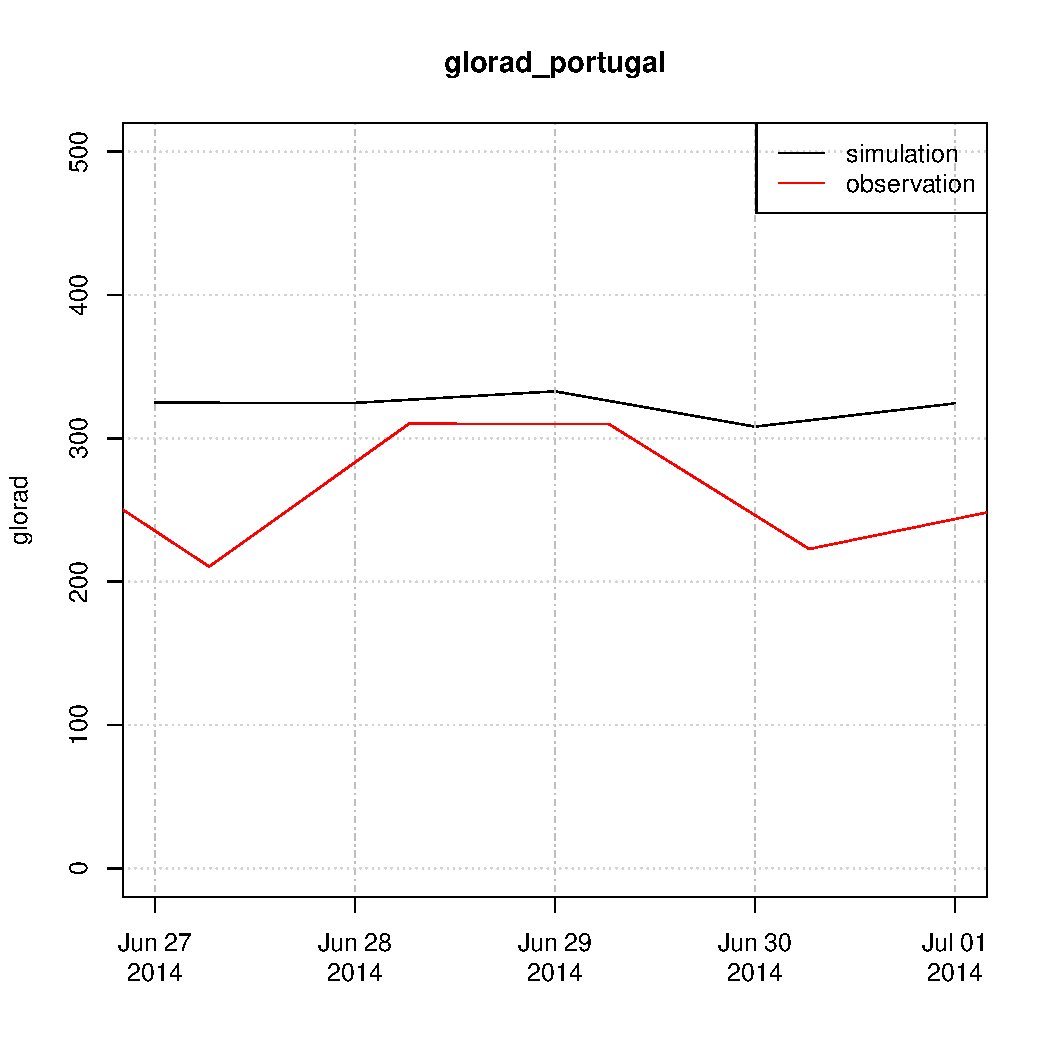
\includegraphics[width=0.8\hsize]{./plot_glorad_compare_portugal_HS_2014-06-26_2014-07-01.pdf}
  \caption{.}
  \label{fig:portugal_HS_glorad1}
\end{figure}

\begin{figure}[ht]
  \centering
  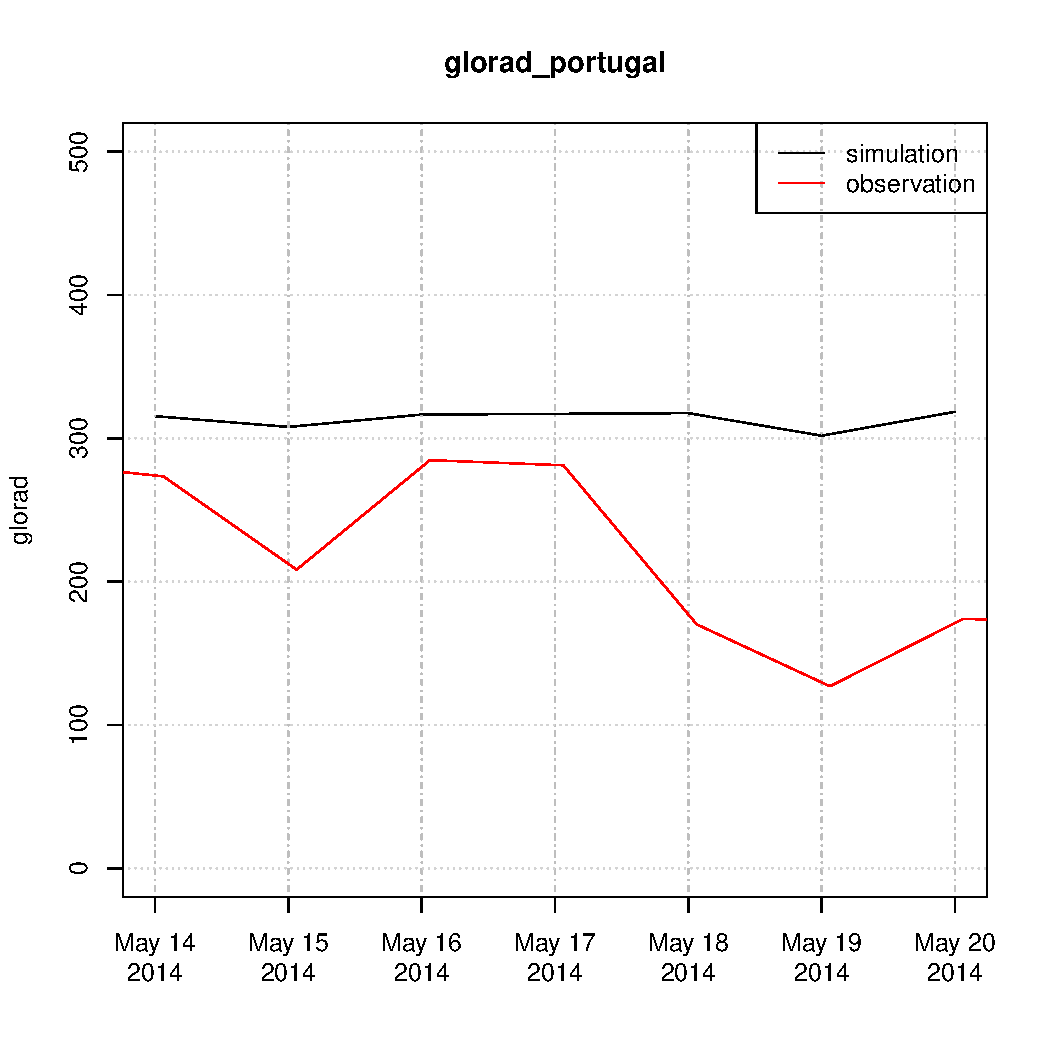
\includegraphics[width=0.8\hsize]{./plot_glorad_compare_portugal_NSA_2014-05-13_2014-05-20.pdf}
  \caption{.}
  \label{fig:portugal_NSA_glorad1}
\end{figure}

\subsection{\texttt{glorad}: Morocco}

\section{Net incoming radiation \texttt{rad\_net}}

\subsection{\texttt{rad\_net}: Portugal}

\begin{figure}[ht]
  \centering
  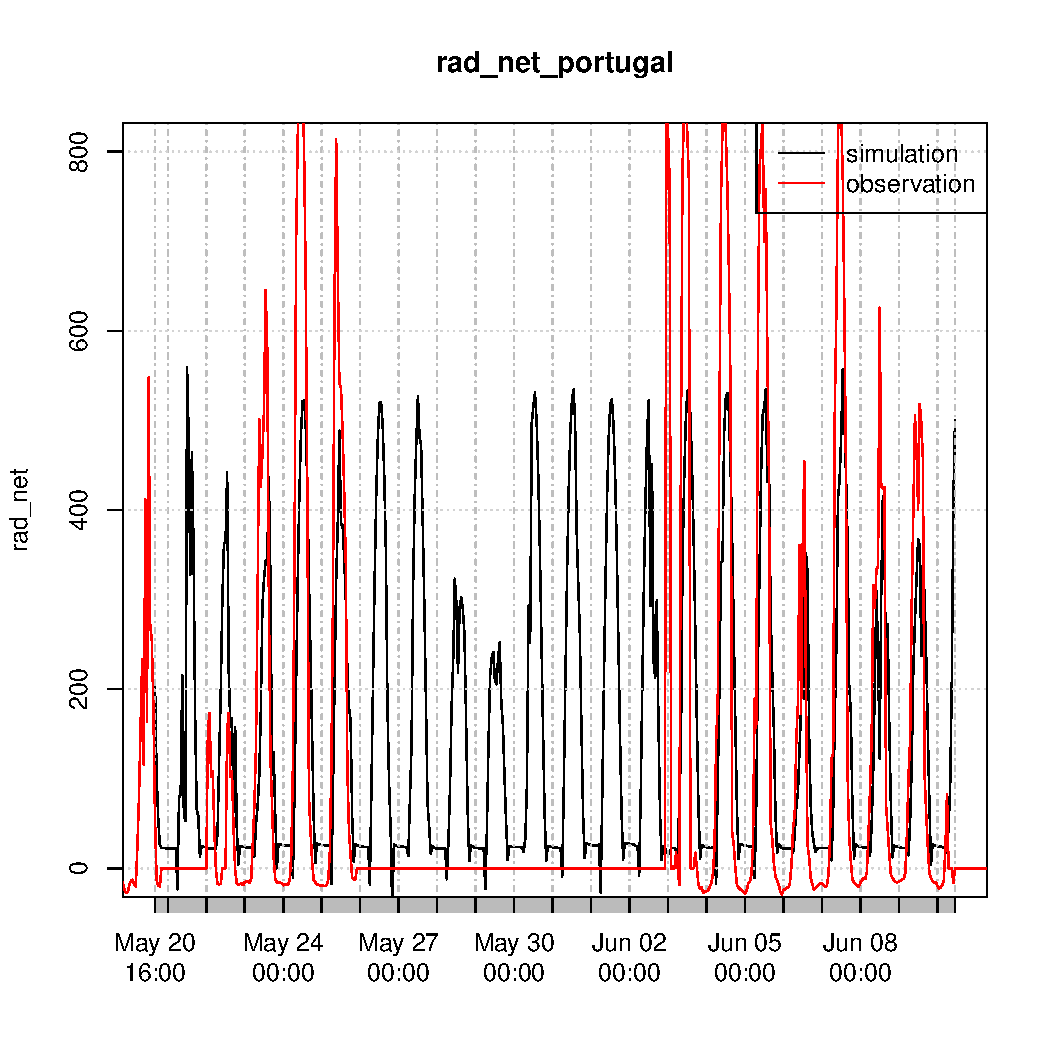
\includegraphics[width=0.8\hsize]{./plot_rad_net_compare_portugal_HS_2014-04-29_2014-07-01.pdf}
  \caption{.}
  \label{fig:portugal_HS_radnet1}
\end{figure}

\begin{figure}[ht]
  \centering
  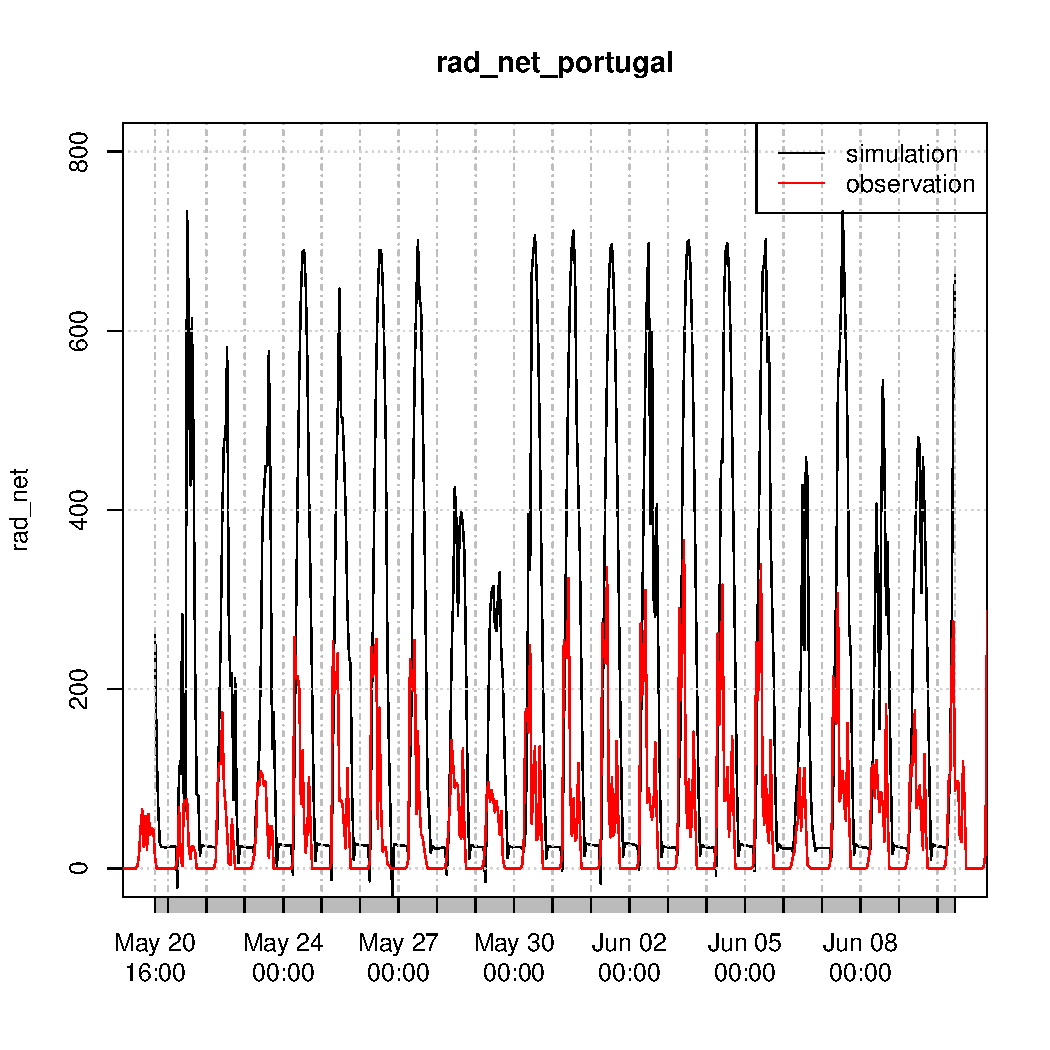
\includegraphics[width=0.8\hsize]{./plot_rad_net_compare_portugal_NSA_2014-04-29_2014-07-01.pdf}
  \caption{.}
  \label{fig:portugal_NSA_radnet1}
\end{figure}

\section{Soilheat flux \texttt{soilheat}}

\subsection{\texttt{soilheat}: Portugal}

\begin{figure}[ht]
  \centering
  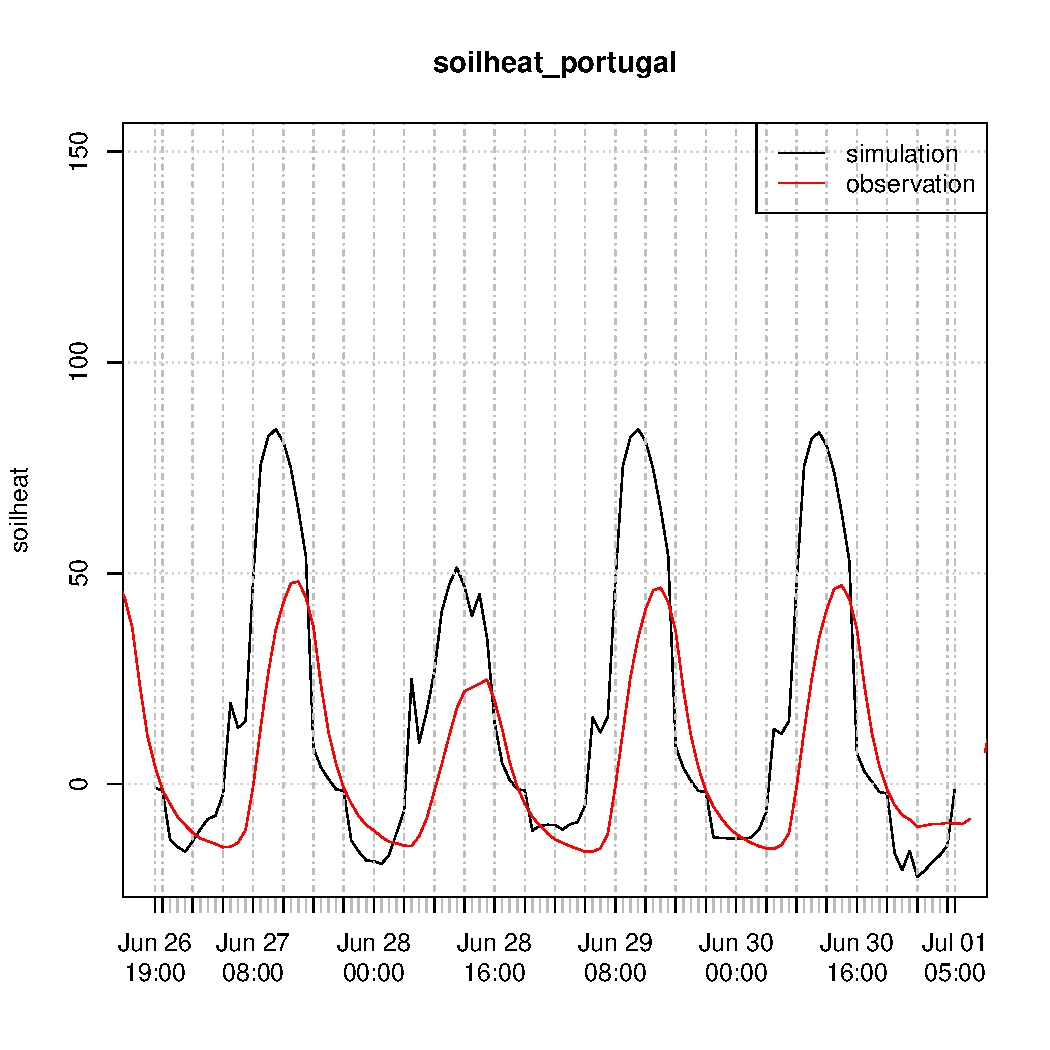
\includegraphics[width=0.8\hsize]{./plot_soilheat_compare_portugal_HS_2014-06-26_2014-07-01.pdf}
  \caption{.}
  \label{fig:portugal_HS_soilheat1}
\end{figure}

\begin{figure}[ht]
  \centering
  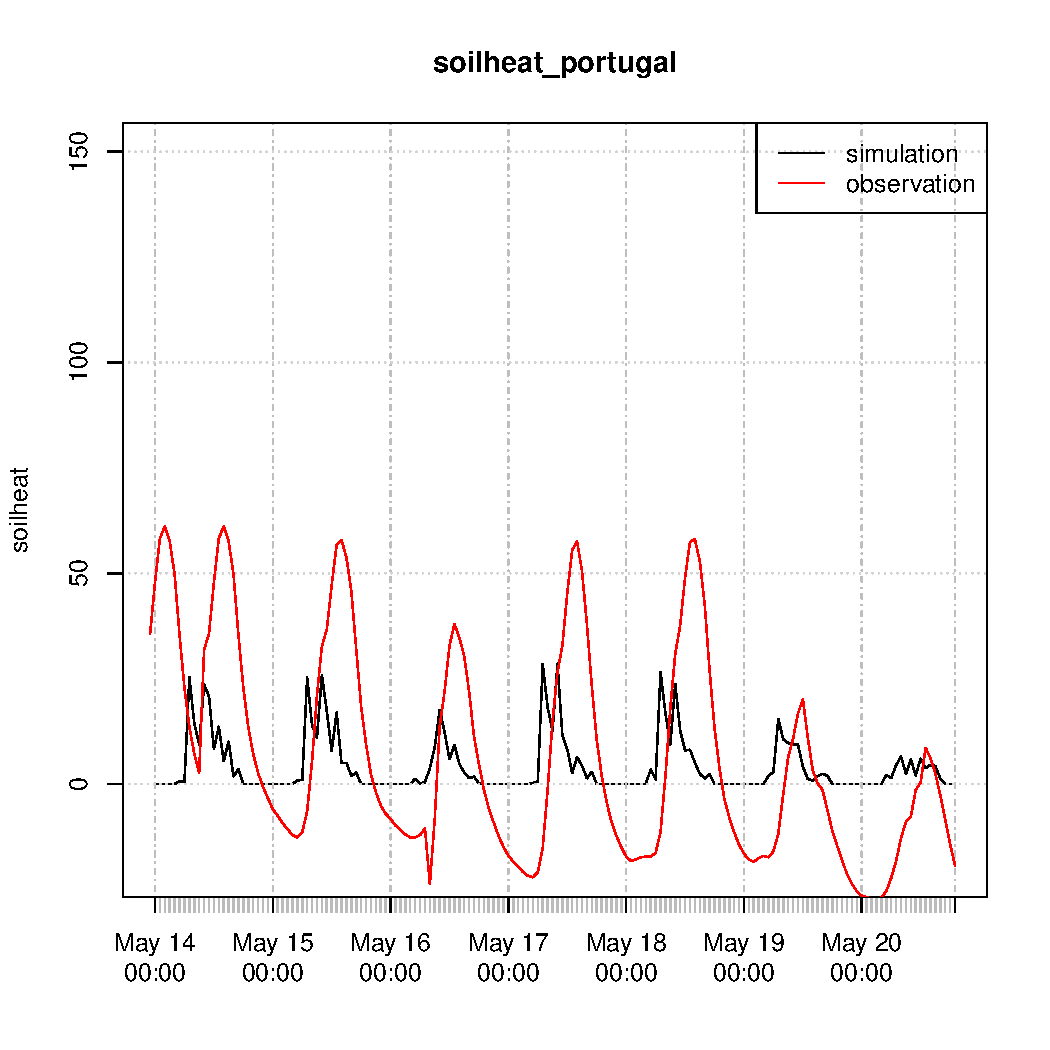
\includegraphics[width=0.8\hsize]{./plot_soilheat_compare_portugal_NSA_2014-05-13_2014-05-20.pdf}
  \caption{.}
  \label{fig:portugal_NSA_soilheat1}
\end{figure}


%................................................................................

\chapter{Results: overview} \label{ch:results}

\section{Parameters} \label{sec:results_par}

An overview of the parameters is given for the \textsf{paramNum} group (object-specific scalar parameters, HS Portugal: Tab. \ref{tab:portugalHS_paramNum}, NSA Portugal: Tab. \ref{tab:portugalNSA_paramNum}, Morocco: Tab.), the \textsf{sharedParamNum} group (group-specific scalar parameters, HS Portugal: Tab. \ref{tab:portugalHS_sharedParamNum}, NSA Portugal: Tab. \ref{tab:portugalNSA_sharedParamNum}, Morocco: Tab.), and the \textsf{inputExt} group (group-specific scalar parameters given as time series, HS Portugal: Tab. \ref{tab:portugalHS_inputExt}, NSA Portugal: Tab. \ref{tab:portugalNSA_inputExt}, Morocco: Tab.).

% latex table generated in R 3.2.2 by xtable 1.8-2 package
% Fri May 12 11:06:02 2017
\begin{table}[ht]
\centering
\caption{Object-specific scalar parameters (\textsf{paramNum}), HS Portugal} 
\label{tab:portugalHS_paramNum}
\begin{tabular}{lrll}
  \hline
Parameter & Value & Unit & Comment \\ 
  \hline
\verb!bubble! & 8.08 & hPa & PTF by \citet{rawls85} \\ 
  \verb!crop_faoref! & 1.00 & -- & evaporation of reference crop \\ 
  \verb!crop_makk! & 0.80 & -- & Eq. \eqref{eq:cropmakk} \\ 
  \verb!elev! & 160.00 & m & local elevation map \\ 
  \verb!glo_half! & 200.00 & W m$^{-2}$ & guessed \\ 
  \verb!lat! & 39.14 & ° & GIS data \\ 
  \verb!lon! & 8.33 & ° & ditto \\ 
  \verb!par_stressHum! & 0.03 & hPa$^{-1}$ & guessed \\ 
  \verb!pores_ind! & 0.45 & -- & PTF by \citet{rawls85} \\ 
  \verb!res_leaf_min! & 50.00 & s m$^{-1}$ & guessed \\ 
  \verb!soil_dens! & 1500.00 & kg m$^{-3}$ & guessed \\ 
  \verb!wc_etmax! & 0.13 & -- & calibration \\ 
  \verb!wc_pwp! & 0.07 & -- & PTF by \citet{rawls85} \\ 
  \verb!wc_res! & 0.05 & -- & (PTF by \citet{rawls85}) \\ 
  \verb!wc_sat! & 0.39 & -- & PTF by \citet{woesten99} \\ 
  \verb!wstressmax! & 10000.00 & hPa & wilting point \\ 
  \verb!wstressmin! & 100.00 & hPa & field capacity \\ 
   \hline
\end{tabular}
\end{table}


% latex table generated in R 3.3.1 by xtable 1.8-2 package
% Fri Jun 23 13:13:45 2017
\begin{table}[ht]
\centering
\caption{Object-specific scalar parameters (\textsf{paramNum}), NSA Portugal} 
\label{tab:portugalNSA_paramNum}
\begin{tabular}{lrll}
  \hline
Parameter & Value & Unit & Comment \\ 
  \hline
\verb!bubble! & 8.08 & hPa & PTF by \citet{rawls85} \\ 
  \verb!crop_faoref! & 1.00 & -- & evaporation of reference crop \\ 
  \verb!crop_makk! & 0.51 & -- & Eq. \eqref{eq:cropmakk} \\ 
  \verb!elev! & 160.00 & m & local elevation map \\ 
  \verb!glo_half! & 200.00 & W m$^{-2}$ & guessed \\ 
  \verb!lat! & 39.14 & ° & GIS data \\ 
  \verb!lon! & 8.33 & ° & ditto \\ 
  \verb!par_stressHum! & 0.03 & hPa$^{-1}$ & guessed \\ 
  \verb!pores_ind! & 0.45 & -- & PTF by \citet{rawls85} \\ 
  \verb!res_leaf_min! & 50.00 & s m$^{-1}$ & guessed \\ 
  \verb!soil_dens! & 1500.00 & kg m$^{-3}$ & guessed \\ 
  \verb!wc_etmax! & 0.13 & -- & calibration \\ 
  \verb!wc_pwp! & 0.07 & -- & PTF by \citet{rawls85} \\ 
  \verb!wc_res! & 0.05 & -- & (PTF by \citet{rawls85}) \\ 
  \verb!wc_sat! & 0.39 & -- & PTF by \citet{woesten99} \\ 
  \verb!wstressmax! & 13100.00 & hPa & wilting point \\ 
  \verb!wstressmin! & 100.00 & hPa & field capacity \\ 
   \hline
\end{tabular}
\end{table}


% latex table generated in R 3.3.1 by xtable 1.8-2 package
% Mon Feb 13 13:53:26 2017
\begin{table}[ht]
\centering
\caption{Group-specific scalar parameters (\textsf{sharedParamNum}), HS Portugal} 
\label{tab:portugalHS_sharedParamNum}
\begin{tabular}{lrll}
  \hline
Parameter & Value & Unit & Comment \\ 
  \hline
\verb!drag_coef! & 0.07 & -- & calibration \\ 
  \verb!eddy_decay! & 2.50 & -- & as used by \citet{shuttleworth85} from \citet{monteith73} \\ 
  \verb!emis_a! & 0.34 & -- & as used by \citet{maidment93} for average conditions \\ 
  \verb!emis_b! & -0.14 & -- & ditto \\ 
  \verb!ext! & 0.40 & -- & guessed \\ 
  \verb!f_day! & 0.14 & -- & estimation from soil heat data \\ 
  \verb!f_night! & 0.49 & -- & ditto \\ 
  \verb!fcorr_a! & 1.35 & -- & as used by \citet{maidment93} \\ 
  \verb!fcorr_b! & -0.35 & -- & ditto \\ 
  \verb!h_humMeas! & 2.00 & m &  \\ 
  \verb!h_tempMeas! & 2.00 & m &  \\ 
  \verb!h_windMeas! & 2.00 & m &  \\ 
  \verb!radex_a! & 0.14 & -- & estimation from radiation data \\ 
  \verb!radex_b! & 0.67 & -- & ditto \\ 
  \verb!res_b! & 25.00 & s m$^{-1}$ & as used by \citet{shuttleworth85} \\ 
  \verb!rough_bare! & 0.01 & m & ditto \\ 
  \verb!rss_a! & 37.50 & -- &  \\ 
  \verb!rss_b! & -1.23 & -- &  \\ 
   \hline
\end{tabular}
\end{table}


% latex table generated in R 3.3.1 by xtable 1.8-2 package
% Wed Dec 14 20:44:30 2016
\begin{table}[ht]
\centering
\caption{Group-specific scalar parameters (\textsf{sharedParamNum}), NSA Portugal} 
\label{tab:portugalNSA_sharedParamNum}
\begin{tabular}{lrll}
  \hline
Parameter & Value & Unit & Comment \\ 
  \hline
\verb!drag_coef! & 0.07 & -- & calibration \\ 
  \verb!eddy_decay! & 2.50 & -- & as used by \citet{shuttleworth85} from \citet{monteith73} \\ 
  \verb!emis_a! & 0.34 & -- & as used by \citet{maidment93} for average conditions \\ 
  \verb!emis_b! & -0.14 & -- & ditto \\ 
  \verb!ext! & 0.40 & -- & guessed \\ 
  \verb!f_day! & 0.10 & -- & estimation from soil heat data \\ 
  \verb!f_night! & 0.70 & -- & ditto \\ 
  \verb!fcorr_a! & 1.35 & -- & as used by \citet{maidment93} \\ 
  \verb!fcorr_b! & -0.35 & -- & ditto \\ 
  \verb!h_humMeas! & 4.84 & m &  \\ 
  \verb!h_tempMeas! & 4.84 & m &  \\ 
  \verb!h_windMeas! & 4.84 & m &  \\ 
  \verb!radex_a! & 0.14 & -- & estimation from radiation data \\ 
  \verb!radex_b! & 0.67 & -- & ditto \\ 
  \verb!res_b! & 25.00 & s m$^{-1}$ & as used by \citet{shuttleworth85} \\ 
  \verb!rough_bare! & 0.01 & m & ditto \\ 
  \verb!rss_a! & 37.50 & -- &  \\ 
  \verb!rss_b! & -1.23 & -- &  \\ 
   \hline
\end{tabular}
\end{table}


% latex table generated in R 3.2.2 by xtable 1.8-2 package
% Fri May 19 10:20:10 2017
\begin{table}[ht]
\centering
\caption{Time-dependent parameters (\textsf{inputExt}), HS Portugal} 
\label{tab:portugalHS_inputExt}
\begin{tabular}{lrl}
  \hline
Parameter & Value & Unit \\ 
  \hline
\verb!alb! & 0.07 & -- \\ 
  \verb!cano_height! & 0.20 & m \\ 
  \verb!lai! & 0.78 & -- \\ 
   \hline
\end{tabular}
\end{table}


% latex table generated in R 3.3.1 by xtable 1.8-2 package
% Fri May 26 11:49:56 2017
\begin{table}[ht]
\centering
\caption{Time-dependent parameters (\textsf{inputExt}), NSA Portugal} 
\label{tab:portugalNSA_inputExt}
\begin{tabular}{lrl}
  \hline
Parameter & Value & Unit \\ 
  \hline
\verb!alb! & 0.07 & -- \\ 
  \verb!cano_height! & 7.98 & m \\ 
  \verb!lai! & 1.40 & -- \\ 
   \hline
\end{tabular}
\end{table}


%................................................................................

\chapter{Conclusion} \label{ch:conclusion}

The calculation of the soil heat flux could be improved by a simple implementation of the 1-dimensional heat equation using finite differences.
This method would require data of the soil temperature in two different depths and data of the specific heat capacity $c$.
The latter one could also be derived by
%
\begin{align*}
  c = 2.45 \times x_\text{mineral} + 2.45 \times x_\text{org} + 4.186 \times x_\text{water},
\end{align*}
%
with
\begin{denseitem}
  \item[] $x_\text{mineral}$: mass fraction of minerals in the soil, in m$^3$~m$^{-3}$,
  \item[] $x_\text{org}$: mass fraction of organic matter in the soil, in m$^3$~m$^{-3}$,
  \item[] $x_\text{water}$: mass fraction of water in the soil, in m$^3$~m$^{-3}$.
\end{denseitem}

%................................................................................

\bibliography{./jubib}

%................................................................................

\end{document}